
\documentclass[a4paper,12pt]{report}
\usepackage[centertags]{amsmath}
\usepackage{tensor}
\usepackage{amsfonts}
\usepackage{amssymb}
\usepackage{amsthm}
\usepackage{mathtools}
\usepackage{caption}
\usepackage{subcaption}
\usepackage{graphicx}
\usepackage{newlfont}
\usepackage{float}
\usepackage{listings}
\usepackage{xcolor}
\usepackage{hyperref}
\usepackage[utf8]{inputenc}
\usepackage{cite}

\lstset{
    language=Python,
    basicstyle=\ttfamily\small,
    keywordstyle=\color{blue},
    commentstyle=\color{gray},
    stringstyle=\color{orange},
    showstringspaces=false,
    breaklines=true,
    frame=single,
    captionpos=b,
    tabsize=4,
    numbers=left,
    numberstyle=\tiny\color{gray},
    xleftmargin=2em,
    xrightmargin=2em,
    aboveskip=1em,
    belowskip=1em
}

\usepackage[letterpaper, left=1.5in, right=1in, top=1in, bottom=1in]{geometry}
\usepackage{appendix}
\theoremstyle{definition}
\newtheorem{definition}{Definition}[section]
\renewcommand{\baselinestretch}{1.5}

\newcommand{\setlinespacing}[1]%
           {\setlength{\baselineskip}{#1 \defbaselineskip}}
\newcommand{\doublespacing}{\setlength{\baselineskip}%
                           {2.0 \defbaselineskip}}
\newcommand{\singlespacing}{\setlength{\baselineskip}{\defbaselineskip}}
% MATH -------------------------------------------------------------------
\newcommand{\x}{{\mathbf{x}}}
\newcommand{\p}{{\mathbf{p}}}
\newcommand{\q}{{\mathbf{q}}}
\newcommand{\Real}{\mathbb R}
\newcommand{\PR}{(0,\infty)}
\newcommand{\R}{\mathbb{R}}
\newcommand{\N}{\mathbb{N}}
%\newcommand{\example}
% THEOREMS ---------------------------------------------------------------

%\theoremstyle{plain}
\newtheorem{theorem}{Theorem}[chapter]
\newtheorem{corollary}[theorem]{Corollary}
\newtheorem{lemma}[theorem]{Lemma}
\newtheorem{proposition}[theorem]{Proposition}
\newtheorem{example}{Example}[section]
%\newtheorem{figure}{figure}[section]
%
%\theoremstyle{definition}
%
%\theoremstyle{remark}
\newtheorem{remark}{Remark}[section]
%
\numberwithin{equation}{section}
\renewcommand{\theequation}{\thesection.\arabic{equation}}

\usepackage[mathscr]{euscript}
\usepackage[normalem]{ulem}
\usepackage{tocloft}

\renewcommand\cftchapafterpnum{\vskip7pt}
\renewcommand\cftsecafterpnum{\vskip7pt}
%-------------------------------

%Landscape Table

%\usepackage{lscape}
%\usepackage{pdflscape}
%\usepackage{float,lscape}


%Tree Graph
\usepackage{qtree}


%TABLE

%\usepackage[T1]{fontenc}
%\usepackage[utf8]{inputenc}
\usepackage{tabularx,ragged2e,booktabs,caption}
\newcolumntype{C}[1]{>{\Centering}m{#1}}
\renewcommand\tabularxcolumn[1]{C{#1}}\\


\begin{document}

% Title Page
\begin{titlepage}
    \centering
    \vspace*{2cm}
    
    % Title
    {\Large \textbf{Data-driven Modelling and Analysis for Applied Dynamic Systems}} \\[1.5cm]
    
    % Subtitle 
    {\large \textbf{Improved Approach for Implementing Dynamic Mode Decomposition with Control}} \\[1cm]
    {\large \textbf{Project Report}} \\[1cm]
    % Author's Name
    {\large \textbf{Prepared by:}} \\
    {\large \textbf{\textrm{Xuan Nguyen, Swahibath Saad, QuocViet Pham, Ali Mohsin Hussain, Talha Sajid
}}} \\[1cm]

    {\large \textbf{Course Instructor}} \\
    {\large \textbf{\textrm{Sergey Safonov
    }}} \\[1cm]
    
    % Designation and Department
    
    
    
    
    
    \vspace{2cm}
    
    % Institution Logo
     
\includegraphics[width=0.5\textwidth]{Snimok-ekrana-2022-09-19-v-15.24.24-300x103.jpg}  % Add the path to your institution's logo
    
\end{titlepage}

\subsection*{Project Team}
\begin{itemize}
    \item \textbf{QuocViet Pham}: Original Lotka–Volterra ODE equations
    \item \textbf{Talha Sajid}: Original Lorenz ODE system
    \item \textbf{Xuan Nguyen}: Improved Lotka–Volterra and Lorenz systems
    \item \textbf{Ali Mohsin Hussain}:  Altered Lotka–Volterra system
    \item \textbf{Swahibath Saad}:  Altered Lorenz ODE system
\end{itemize}

\subsection*{Background}

This project explores the effectiveness of Dynamic Mode Decomposition with Control (DMDc) in modeling complex nonlinear systems. The focus is on implementing both the standard DMDc algorithm and an improved method that reduces computational cost through lower-order SVD and simpler dynamic mode structure\cite{bai2020}. We apply these techniques to the Lotka–Volterra and Lorenz ODE systems, representing biological and chaotic dynamics. Simulations were performed using Python and SciPy, and snapshot data was used to construct the augmented matrix $\Omega = [X; \Gamma]$\ \cite{dawson2015}. Key techniques include SVD, low-rank truncation, and eigenvalue decomposition to estimate system matrices $A$ and $B$, compute DMD modes $\Phi$, and reconstruct system behavior. Performance was evaluated based on eigenvalue distribution, trajectory reconstruction accuracy, and relative error\cite{fonzi2020}.

\subsection*{Result Summary}
This project applied standard and improved DMDc algorithms to the Lotka–Volterra and Lorenz systems using Python simulations. DMDc was used to extract dynamic modes, estimate system matrices, and reconstruct trajectories\cite{A2}. Results included accurate state reconstructions, stable eigenvalue plots, and low relative errors. The improved method achieved similar accuracy with reduced computation. Both methods performed well, but further work is needed for complex or noisy systems.

\subsubsection*{Original Lotka–Volterra and Lorenz Systems}
The original Lotka–Volterra and Lorenz systems were simulated without control inputs. Standard DMDc was applied using a zero control matrix, and the reconstructed results closely matched the true dynamics, confirming the method’s effectiveness for uncontrolled systems\cite{liew2022}.

\begin{figure}[h!]
    \centering
    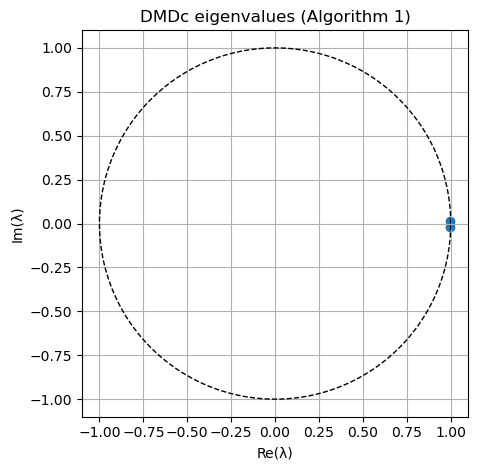
\includegraphics[width=0.27\textwidth]{OELV.png}\hspace{2cm}
    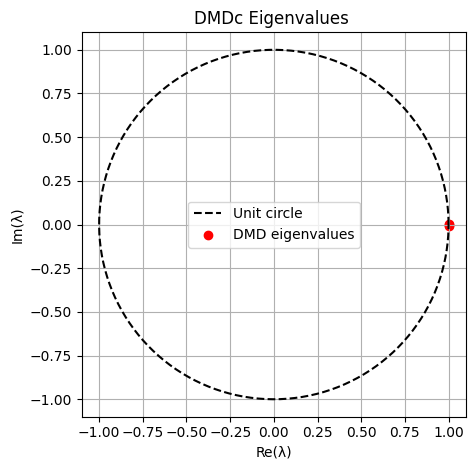
\includegraphics[width=0.27\textwidth]{OEL.png}
    \caption{Eigenvalues (Lotka–Volterra) and Lorenz attractor.}

\end{figure}
\begin{figure}[h!]
    \centering
    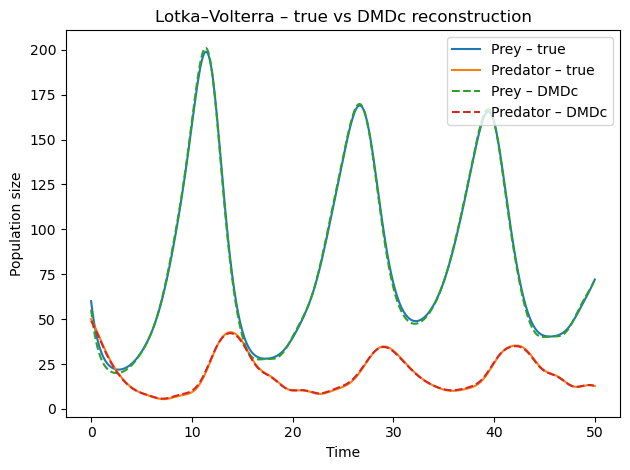
\includegraphics[width=0.27\textwidth]{OLV.png}\hspace{2cm}
    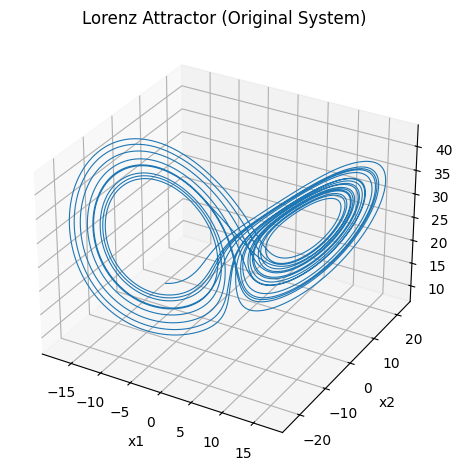
\includegraphics[width=0.27\textwidth]{OLA.png}
    \caption{Lotka–Volterra: True vs DMDc and altered system results.}
\end{figure}
\begin{figure}[h!]
    \centering
    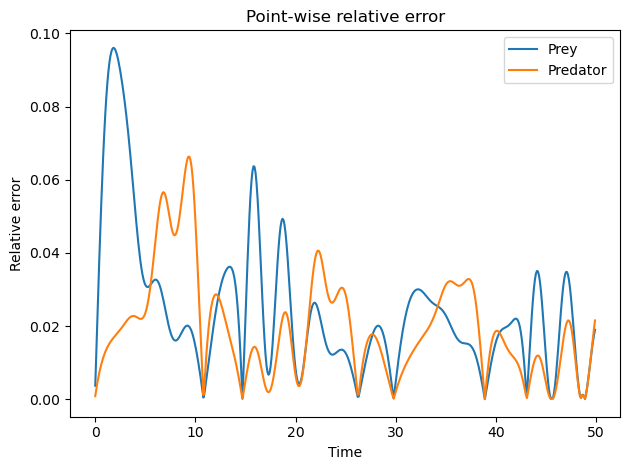
\includegraphics[width=0.3\textwidth]{POINTWISE LV.png}\hspace{1cm}
    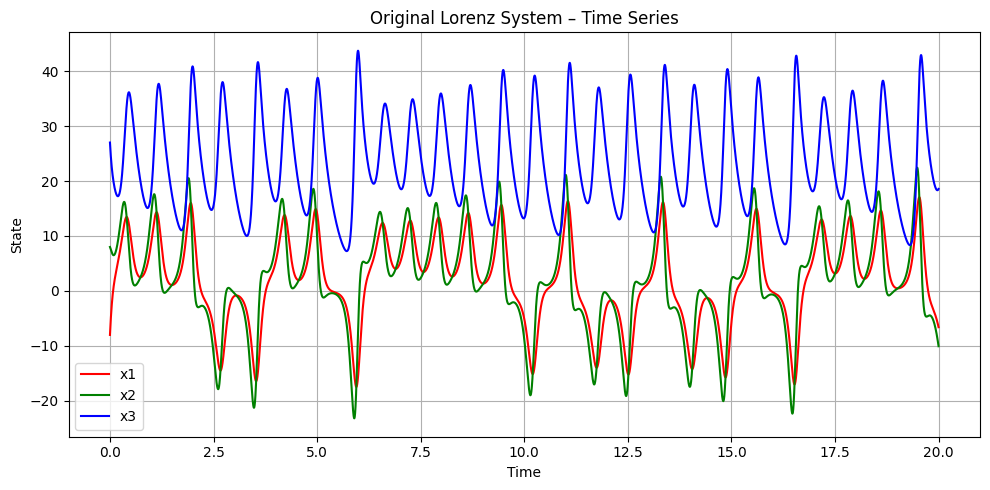
\includegraphics[width=0.45\textwidth]{OLT.png}
   \caption{Relative error (Lotka–Volterra) and Lorenz time series.}
\end{figure}
\newpage
\subsubsection*{Improved DMDc Method}

The improved DMDc algorithm reduces computation using lower-rank SVD while maintaining accuracy. It achieved efficient trajectory reconstruction and stable eigenvalue results on both systems\cite{proctor2018}.
% Figure 1: Improved Lorenz
\begin{figure}[h!]
    \centering
    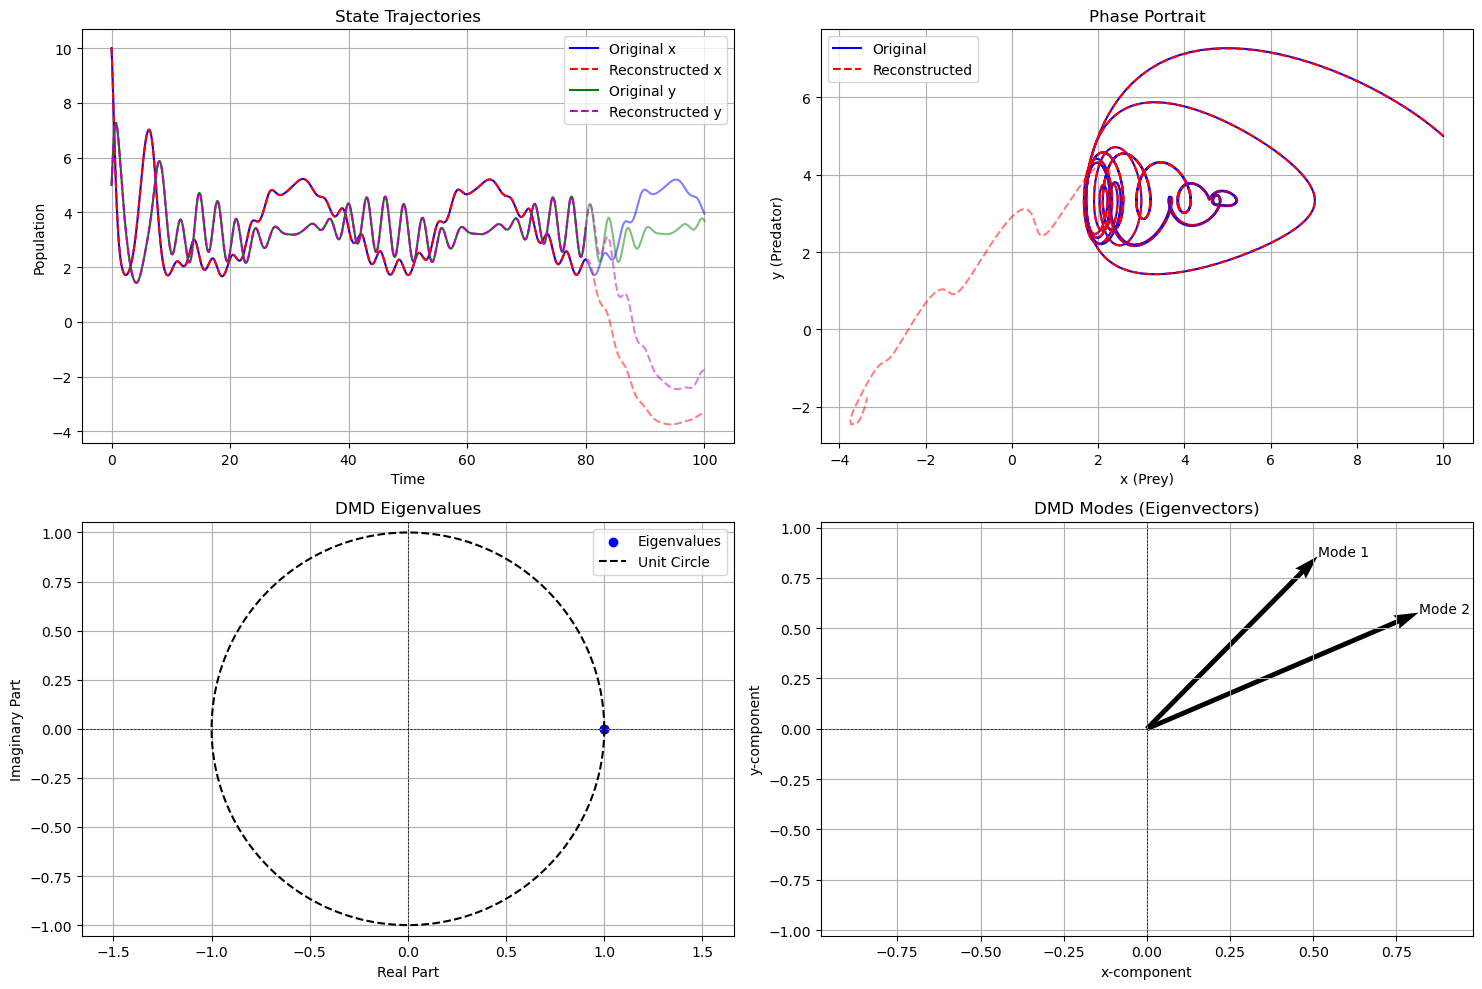
\includegraphics[width=0.75\textwidth]{IPROVED LV.png}
    
    \vspace{1em}
    
    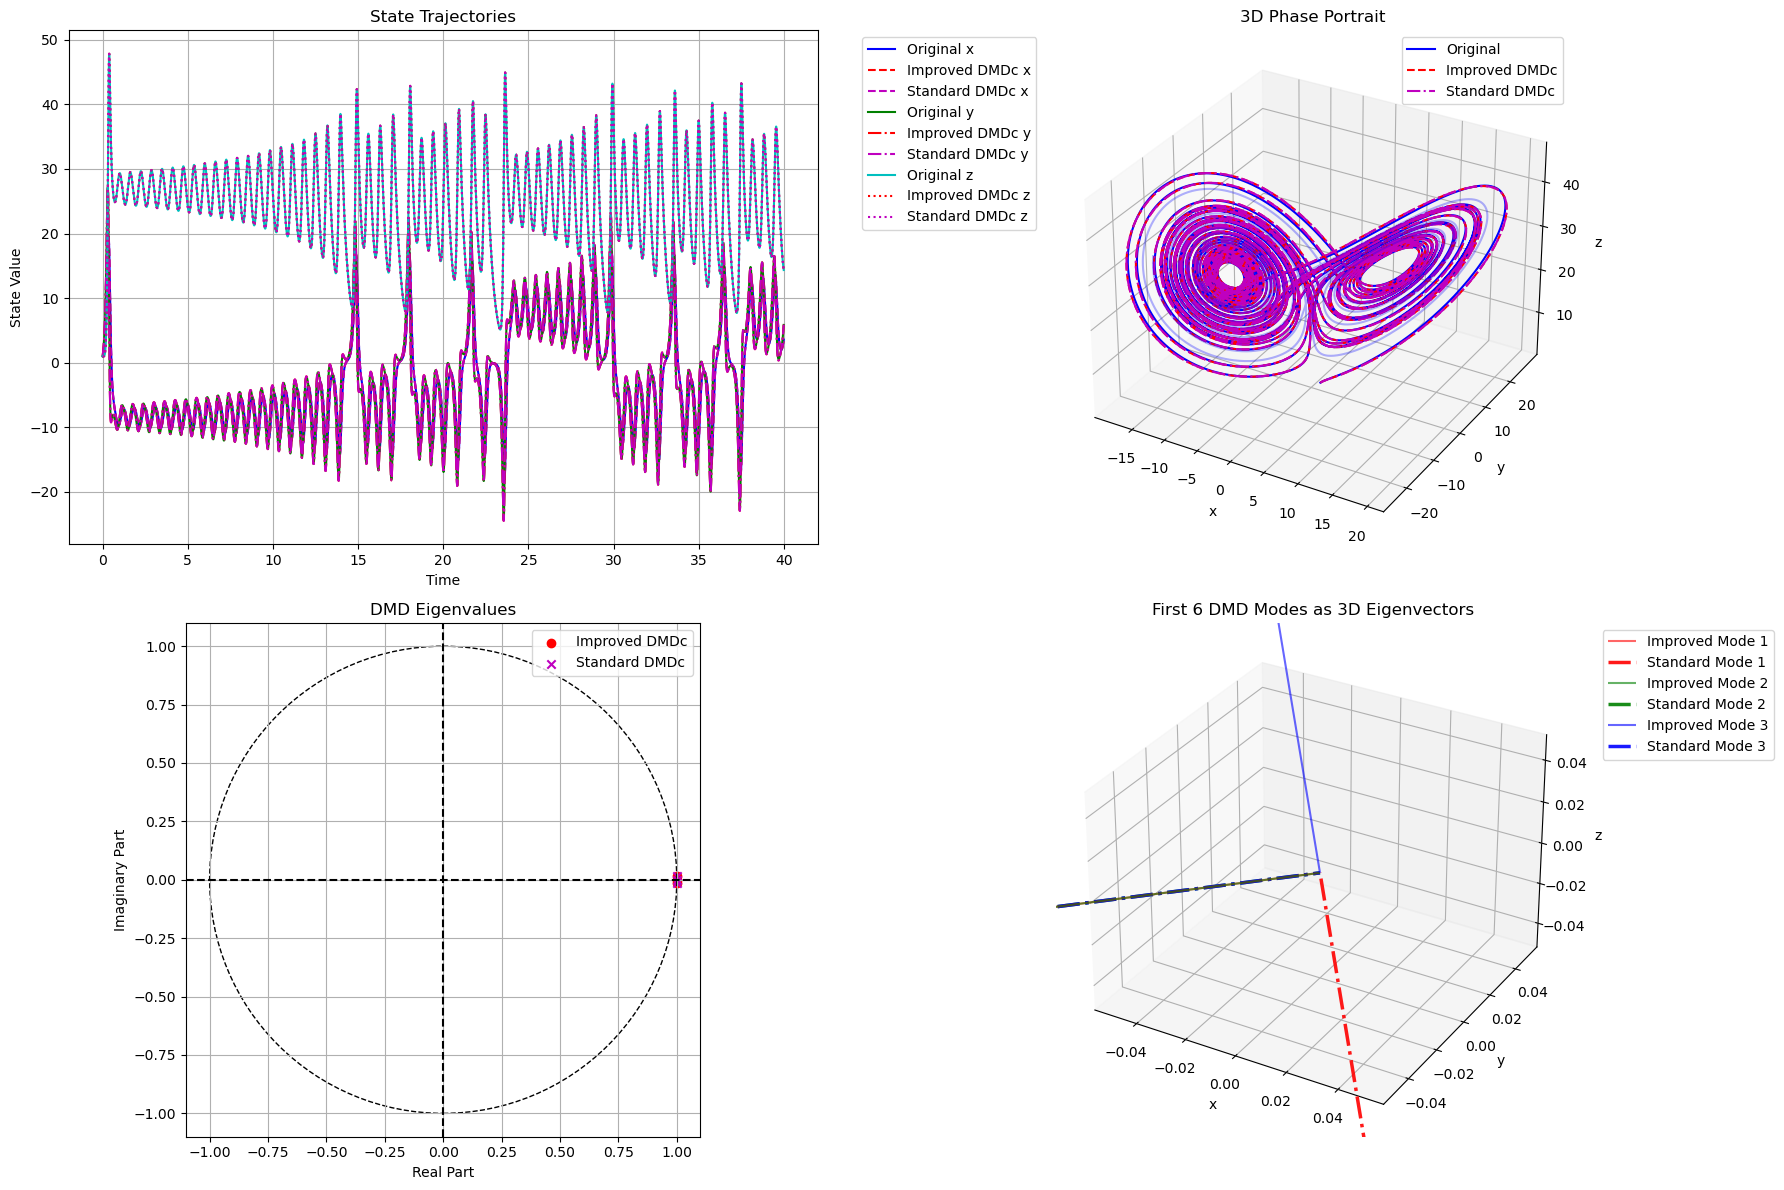
\includegraphics[width=0.75\textwidth]{IMPROVED LORENZ.png}
    
    \caption{Improved DMDc results. Top: Lotka–Volterra system showing trajectories, phase portrait, eigenvalues, and DMD modes. Bottom: Lorenz system with corresponding outputs including 3D attractor and eigenvalue distribution.}
\end{figure}



\newpage
\subsubsection*{Alternative Systems}

The altered Lotka–Volterra and Lorenz systems introduced changes to test the robustness of DMDc methods. Both standard and improved algorithms maintained good reconstruction accuracy, with the improved method remaining more efficient\cite{swaminathan2022}.
\begin{figure}[h!]
    \centering
    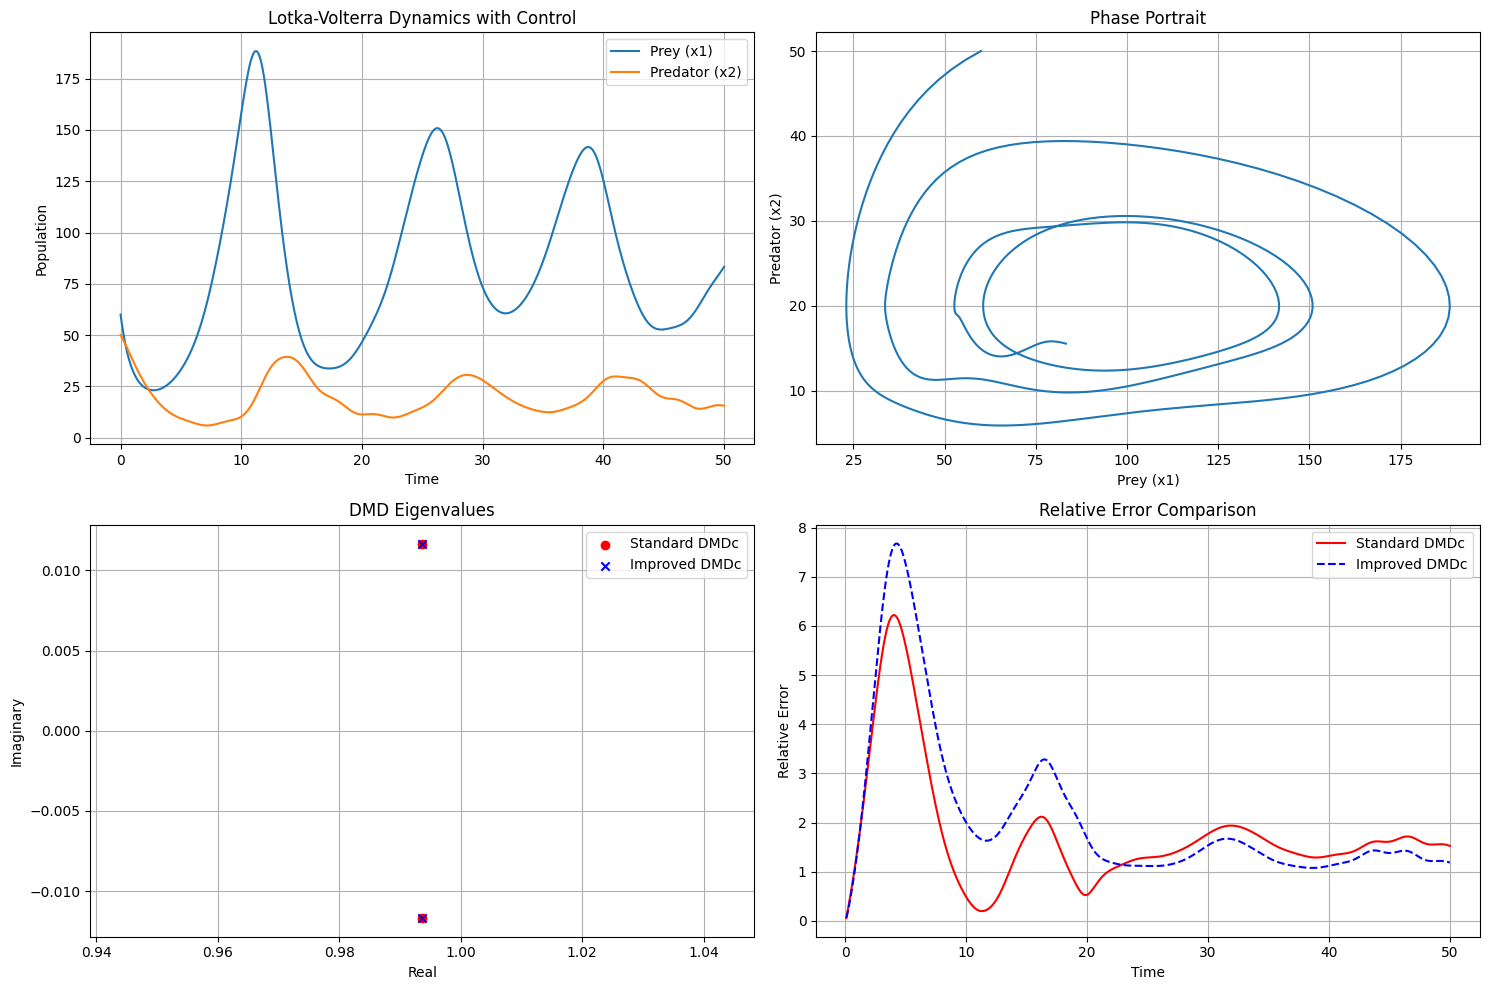
\includegraphics[width=0.5\textwidth]{Alter lv.png}
    
    \vspace{1em}
    
    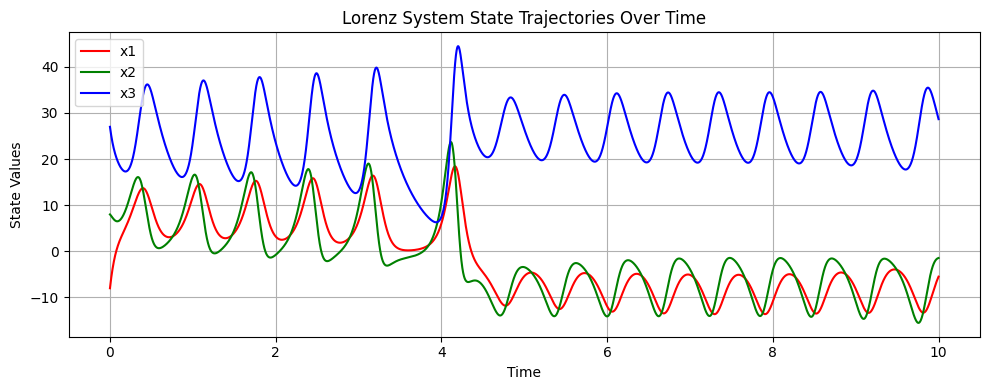
\includegraphics[width=0.5\textwidth]{ALTER LODE.png}
    
    \vspace{1em}
    
    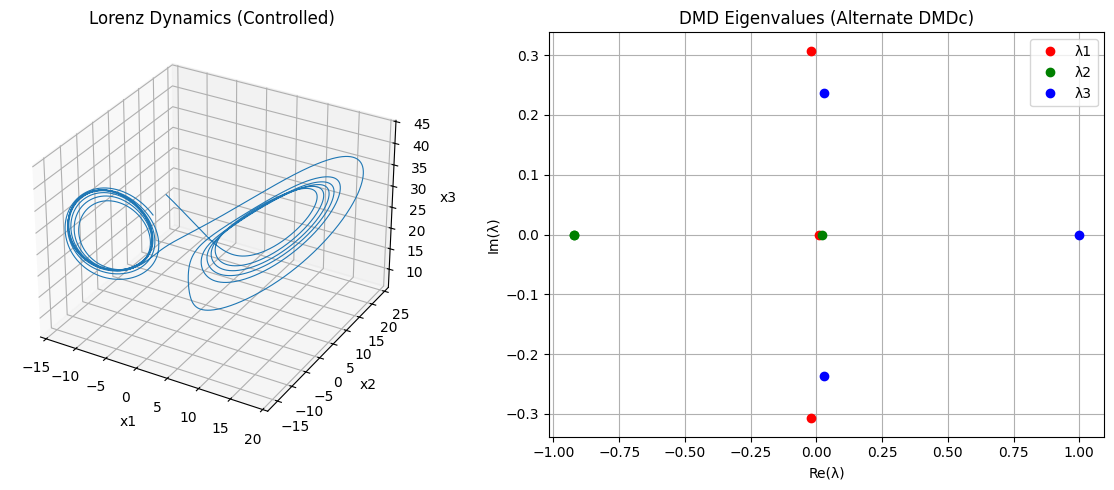
\includegraphics[width=0.65\textwidth]{ALTER L.png}
    
    \caption{Altered system results. Top: Lotka–Volterra – reconstructed vs true dynamics under modified conditions. Middle and bottom: Lorenz system – controlled dynamics, eigenvalue plot, and time-series of $x_1$, $x_2$, and $x_3$.}
\end{figure}\\
The project code and implementation are available at: 
\href{https://github.com/thexuanphuc/impoved_DMDC/tree/master}{GitHub Repository}.

\newpage
\renewcommand{\bibname}{References}
\begingroup
\small
\bibliographystyle{plain}
\bibliography{reference}
\endgroup
























































































































































































\end{document}













































































































































































































































\end{document}